% Options for packages loaded elsewhere
\PassOptionsToPackage{unicode}{hyperref}
\PassOptionsToPackage{hyphens}{url}
%
\documentclass[
]{article}
\usepackage{amsmath,amssymb}
\usepackage{iftex}
\ifPDFTeX
  \usepackage[T1]{fontenc}
  \usepackage[utf8]{inputenc}
  \usepackage{textcomp} % provide euro and other symbols
\else % if luatex or xetex
  \usepackage{unicode-math} % this also loads fontspec
  \defaultfontfeatures{Scale=MatchLowercase}
  \defaultfontfeatures[\rmfamily]{Ligatures=TeX,Scale=1}
\fi
\usepackage{lmodern}
\ifPDFTeX\else
  % xetex/luatex font selection
\fi
% Use upquote if available, for straight quotes in verbatim environments
\IfFileExists{upquote.sty}{\usepackage{upquote}}{}
\IfFileExists{microtype.sty}{% use microtype if available
  \usepackage[]{microtype}
  \UseMicrotypeSet[protrusion]{basicmath} % disable protrusion for tt fonts
}{}
\makeatletter
\@ifundefined{KOMAClassName}{% if non-KOMA class
  \IfFileExists{parskip.sty}{%
    \usepackage{parskip}
  }{% else
    \setlength{\parindent}{0pt}
    \setlength{\parskip}{6pt plus 2pt minus 1pt}}
}{% if KOMA class
  \KOMAoptions{parskip=half}}
\makeatother
\usepackage{xcolor}
\usepackage[margin=1in]{geometry}
\usepackage{color}
\usepackage{fancyvrb}
\newcommand{\VerbBar}{|}
\newcommand{\VERB}{\Verb[commandchars=\\\{\}]}
\DefineVerbatimEnvironment{Highlighting}{Verbatim}{commandchars=\\\{\}}
% Add ',fontsize=\small' for more characters per line
\usepackage{framed}
\definecolor{shadecolor}{RGB}{248,248,248}
\newenvironment{Shaded}{\begin{snugshade}}{\end{snugshade}}
\newcommand{\AlertTok}[1]{\textcolor[rgb]{0.94,0.16,0.16}{#1}}
\newcommand{\AnnotationTok}[1]{\textcolor[rgb]{0.56,0.35,0.01}{\textbf{\textit{#1}}}}
\newcommand{\AttributeTok}[1]{\textcolor[rgb]{0.13,0.29,0.53}{#1}}
\newcommand{\BaseNTok}[1]{\textcolor[rgb]{0.00,0.00,0.81}{#1}}
\newcommand{\BuiltInTok}[1]{#1}
\newcommand{\CharTok}[1]{\textcolor[rgb]{0.31,0.60,0.02}{#1}}
\newcommand{\CommentTok}[1]{\textcolor[rgb]{0.56,0.35,0.01}{\textit{#1}}}
\newcommand{\CommentVarTok}[1]{\textcolor[rgb]{0.56,0.35,0.01}{\textbf{\textit{#1}}}}
\newcommand{\ConstantTok}[1]{\textcolor[rgb]{0.56,0.35,0.01}{#1}}
\newcommand{\ControlFlowTok}[1]{\textcolor[rgb]{0.13,0.29,0.53}{\textbf{#1}}}
\newcommand{\DataTypeTok}[1]{\textcolor[rgb]{0.13,0.29,0.53}{#1}}
\newcommand{\DecValTok}[1]{\textcolor[rgb]{0.00,0.00,0.81}{#1}}
\newcommand{\DocumentationTok}[1]{\textcolor[rgb]{0.56,0.35,0.01}{\textbf{\textit{#1}}}}
\newcommand{\ErrorTok}[1]{\textcolor[rgb]{0.64,0.00,0.00}{\textbf{#1}}}
\newcommand{\ExtensionTok}[1]{#1}
\newcommand{\FloatTok}[1]{\textcolor[rgb]{0.00,0.00,0.81}{#1}}
\newcommand{\FunctionTok}[1]{\textcolor[rgb]{0.13,0.29,0.53}{\textbf{#1}}}
\newcommand{\ImportTok}[1]{#1}
\newcommand{\InformationTok}[1]{\textcolor[rgb]{0.56,0.35,0.01}{\textbf{\textit{#1}}}}
\newcommand{\KeywordTok}[1]{\textcolor[rgb]{0.13,0.29,0.53}{\textbf{#1}}}
\newcommand{\NormalTok}[1]{#1}
\newcommand{\OperatorTok}[1]{\textcolor[rgb]{0.81,0.36,0.00}{\textbf{#1}}}
\newcommand{\OtherTok}[1]{\textcolor[rgb]{0.56,0.35,0.01}{#1}}
\newcommand{\PreprocessorTok}[1]{\textcolor[rgb]{0.56,0.35,0.01}{\textit{#1}}}
\newcommand{\RegionMarkerTok}[1]{#1}
\newcommand{\SpecialCharTok}[1]{\textcolor[rgb]{0.81,0.36,0.00}{\textbf{#1}}}
\newcommand{\SpecialStringTok}[1]{\textcolor[rgb]{0.31,0.60,0.02}{#1}}
\newcommand{\StringTok}[1]{\textcolor[rgb]{0.31,0.60,0.02}{#1}}
\newcommand{\VariableTok}[1]{\textcolor[rgb]{0.00,0.00,0.00}{#1}}
\newcommand{\VerbatimStringTok}[1]{\textcolor[rgb]{0.31,0.60,0.02}{#1}}
\newcommand{\WarningTok}[1]{\textcolor[rgb]{0.56,0.35,0.01}{\textbf{\textit{#1}}}}
\usepackage{graphicx}
\makeatletter
\def\maxwidth{\ifdim\Gin@nat@width>\linewidth\linewidth\else\Gin@nat@width\fi}
\def\maxheight{\ifdim\Gin@nat@height>\textheight\textheight\else\Gin@nat@height\fi}
\makeatother
% Scale images if necessary, so that they will not overflow the page
% margins by default, and it is still possible to overwrite the defaults
% using explicit options in \includegraphics[width, height, ...]{}
\setkeys{Gin}{width=\maxwidth,height=\maxheight,keepaspectratio}
% Set default figure placement to htbp
\makeatletter
\def\fps@figure{htbp}
\makeatother
\setlength{\emergencystretch}{3em} % prevent overfull lines
\providecommand{\tightlist}{%
  \setlength{\itemsep}{0pt}\setlength{\parskip}{0pt}}
\setcounter{secnumdepth}{-\maxdimen} % remove section numbering
\ifLuaTeX
  \usepackage{selnolig}  % disable illegal ligatures
\fi
\usepackage{bookmark}
\IfFileExists{xurl.sty}{\usepackage{xurl}}{} % add URL line breaks if available
\urlstyle{same}
\hypersetup{
  pdftitle={Week\_1\_Assignment-Data\_608},
  pdfauthor={Mubashira Qari},
  hidelinks,
  pdfcreator={LaTeX via pandoc}}

\title{Week\_1\_Assignment-Data\_608}
\author{Mubashira Qari}
\date{2024-12-21}

\begin{document}
\maketitle

\subsubsection{Load Libraries}\label{load-libraries}

\begin{Shaded}
\begin{Highlighting}[]
\FunctionTok{library}\NormalTok{(tidyverse)}
\end{Highlighting}
\end{Shaded}

\begin{verbatim}
## -- Attaching core tidyverse packages ------------------------ tidyverse 2.0.0 --
## v dplyr     1.1.4     v readr     2.1.5
## v forcats   1.0.0     v stringr   1.5.1
## v ggplot2   3.4.4     v tibble    3.2.1
## v lubridate 1.9.3     v tidyr     1.3.1
## v purrr     1.0.2     
## -- Conflicts ------------------------------------------ tidyverse_conflicts() --
## x dplyr::filter() masks stats::filter()
## x dplyr::lag()    masks stats::lag()
## i Use the conflicted package (<http://conflicted.r-lib.org/>) to force all conflicts to become errors
\end{verbatim}

\begin{Shaded}
\begin{Highlighting}[]
\FunctionTok{library}\NormalTok{(readxl)}
\FunctionTok{library}\NormalTok{(ggplot2)}
\FunctionTok{library}\NormalTok{(dplyr)}
\FunctionTok{library}\NormalTok{(stringr)}
\FunctionTok{library}\NormalTok{(tools)}
\FunctionTok{library}\NormalTok{(stringdist)}
\end{Highlighting}
\end{Shaded}

\begin{verbatim}
## Warning: package 'stringdist' was built under R version 4.3.3
\end{verbatim}

\begin{verbatim}
## 
## Attaching package: 'stringdist'
## 
## The following object is masked from 'package:tidyr':
## 
##     extract
\end{verbatim}

\begin{Shaded}
\begin{Highlighting}[]
\NormalTok{IIJA\_funding\_data }\OtherTok{\textless{}{-}} \FunctionTok{read.csv}\NormalTok{(}\StringTok{"https://raw.githubusercontent.com/uzmabb182/Data\_608/refs/heads/main/Week\%201/IIJA\%20FUNDING\%20AS\%20OF\%20MARCH\%202023.csv"}\NormalTok{)}

\NormalTok{state\_population\_data }\OtherTok{\textless{}{-}} \FunctionTok{read.csv}\NormalTok{(}\StringTok{"https://raw.githubusercontent.com/uzmabb182/Data\_608/refs/heads/main/Week\%201/State\_Population\_Data.csv"}\NormalTok{)}


\NormalTok{election\_results\_2020\_data }\OtherTok{\textless{}{-}} \FunctionTok{read.csv}\NormalTok{(}\StringTok{"https://raw.githubusercontent.com/uzmabb182/Data\_608/refs/heads/main/Week\%201/2020\_Presidential\_Election\_Results.csv"}\NormalTok{)}
\end{Highlighting}
\end{Shaded}

\subsubsection{View the First Few Rows of
Data}\label{view-the-first-few-rows-of-data}

\begin{Shaded}
\begin{Highlighting}[]
\CommentTok{\#print(IIJA\_funding\_data)}
\end{Highlighting}
\end{Shaded}

\begin{Shaded}
\begin{Highlighting}[]
\CommentTok{\# Check column names}
\FunctionTok{colnames}\NormalTok{(IIJA\_funding\_data)}
\end{Highlighting}
\end{Shaded}

\begin{verbatim}
## [1] "State..Teritory.or.Tribal.Nation" "Total..Billions."
\end{verbatim}

\begin{Shaded}
\begin{Highlighting}[]
\CommentTok{\# Renaming the columns}

\NormalTok{IIJA\_funding\_data }\OtherTok{\textless{}{-}}\NormalTok{ IIJA\_funding\_data }\SpecialCharTok{\%\textgreater{}\%}
  \FunctionTok{rename}\NormalTok{(}\AttributeTok{State\_Name =}\NormalTok{ State..Teritory.or.Tribal.Nation, }\AttributeTok{Funding\_Billions =}\NormalTok{ Total..Billions.)}

\CommentTok{\#print(IIJA\_funding\_data)}
\end{Highlighting}
\end{Shaded}

\begin{Shaded}
\begin{Highlighting}[]
\CommentTok{\# Convert column names to lowercase}
\FunctionTok{colnames}\NormalTok{(IIJA\_funding\_data ) }\OtherTok{\textless{}{-}} \FunctionTok{tolower}\NormalTok{(}\FunctionTok{colnames}\NormalTok{(IIJA\_funding\_data ))}

\CommentTok{\# View the modified data frame}
\CommentTok{\#print(IIJA\_funding\_data )}
\end{Highlighting}
\end{Shaded}

\begin{Shaded}
\begin{Highlighting}[]
\CommentTok{\# Sort by population (ascending order)}
\NormalTok{IIJA\_funding\_data }\OtherTok{\textless{}{-}}\NormalTok{ IIJA\_funding\_data[}\FunctionTok{order}\NormalTok{(IIJA\_funding\_data}\SpecialCharTok{$}\NormalTok{state\_name),]}

\CommentTok{\# View the sorted dataframe}
\CommentTok{\#print(IIJA\_funding\_data)}
\end{Highlighting}
\end{Shaded}

\begin{Shaded}
\begin{Highlighting}[]
\CommentTok{\# Replace "Deleware" with "Delaware" conditionally}
\NormalTok{IIJA\_funding\_data}\SpecialCharTok{$}\NormalTok{state\_name[IIJA\_funding\_data}\SpecialCharTok{$}\NormalTok{state\_name }\SpecialCharTok{==} \StringTok{"Deleware"}\NormalTok{] }\OtherTok{\textless{}{-}} \StringTok{"Delaware"}

\CommentTok{\# View the updated DataFrame}
\CommentTok{\#print(IIJA\_funding\_data)}
\end{Highlighting}
\end{Shaded}

\begin{Shaded}
\begin{Highlighting}[]
\CommentTok{\# Add index column using mutate}
\NormalTok{IIJA\_funding\_data }\OtherTok{\textless{}{-}}\NormalTok{ IIJA\_funding\_data }\SpecialCharTok{\%\textgreater{}\%} \FunctionTok{mutate}\NormalTok{(}\AttributeTok{index =} \FunctionTok{row\_number}\NormalTok{())}

\CommentTok{\# View the updated DataFrame}
\CommentTok{\#print(IIJA\_funding\_data)}
\end{Highlighting}
\end{Shaded}

\begin{Shaded}
\begin{Highlighting}[]
\CommentTok{\# Convert first letter of each word to uppercase using str\_to\_title}
\NormalTok{IIJA\_funding\_data}\SpecialCharTok{$}\NormalTok{state\_name }\OtherTok{\textless{}{-}} \FunctionTok{str\_to\_title}\NormalTok{(IIJA\_funding\_data}\SpecialCharTok{$}\NormalTok{state\_name)}

\CommentTok{\# View the updated DataFrame}
\CommentTok{\#print(IIJA\_funding\_data)}
\end{Highlighting}
\end{Shaded}

\begin{Shaded}
\begin{Highlighting}[]
\CommentTok{\# Convert column names to lowercase}
\FunctionTok{colnames}\NormalTok{(state\_population\_data ) }\OtherTok{\textless{}{-}} \FunctionTok{tolower}\NormalTok{(}\FunctionTok{colnames}\NormalTok{(state\_population\_data ))}

\CommentTok{\# View the modified data frame}
\CommentTok{\#print(state\_population\_data)}
\end{Highlighting}
\end{Shaded}

\begin{Shaded}
\begin{Highlighting}[]
\CommentTok{\# Sort by population (ascending order)}
\NormalTok{state\_population\_data }\OtherTok{\textless{}{-}}\NormalTok{ state\_population\_data[}\FunctionTok{order}\NormalTok{(state\_population\_data}\SpecialCharTok{$}\NormalTok{name),]}

\CommentTok{\# View the sorted dataframe}
\CommentTok{\#print(state\_population\_data)}
\end{Highlighting}
\end{Shaded}

\begin{Shaded}
\begin{Highlighting}[]
\CommentTok{\# Convert first letter of each word to uppercase using str\_to\_title}
\NormalTok{state\_population\_data}\SpecialCharTok{$}\NormalTok{name }\OtherTok{\textless{}{-}} \FunctionTok{str\_to\_title}\NormalTok{(state\_population\_data}\SpecialCharTok{$}\NormalTok{name)}

\CommentTok{\# View the updated DataFrame}
\CommentTok{\#print(state\_population\_data)}
\end{Highlighting}
\end{Shaded}

\begin{Shaded}
\begin{Highlighting}[]
\CommentTok{\# Convert column names to lowercase}
\FunctionTok{colnames}\NormalTok{(election\_results\_2020\_data ) }\OtherTok{\textless{}{-}} \FunctionTok{tolower}\NormalTok{(}\FunctionTok{colnames}\NormalTok{(election\_results\_2020\_data ))}

\CommentTok{\# View the modified data frame}
\CommentTok{\#print(election\_results\_2020\_data)}
\end{Highlighting}
\end{Shaded}

\begin{Shaded}
\begin{Highlighting}[]
\CommentTok{\# Convert first letter of each word to uppercase using str\_to\_title}
\NormalTok{election\_results\_2020\_data}\SpecialCharTok{$}\NormalTok{state }\OtherTok{\textless{}{-}} \FunctionTok{str\_to\_title}\NormalTok{(election\_results\_2020\_data}\SpecialCharTok{$}\NormalTok{state)}

\CommentTok{\# View the updated DataFrame}
\CommentTok{\#print(election\_results\_2020\_data)}
\end{Highlighting}
\end{Shaded}

\begin{Shaded}
\begin{Highlighting}[]
\CommentTok{\# Checking datatypes}
\CommentTok{\#str(IIJA\_funding\_data)}

\CommentTok{\#str(election\_results\_2020\_data)}

\DocumentationTok{\#\#\#str(state\_population\_data)}
\end{Highlighting}
\end{Shaded}

\begin{Shaded}
\begin{Highlighting}[]
\CommentTok{\# Convert \textquotesingle{}state\textquotesingle{} column from integer to character}
\NormalTok{state\_population\_data}\SpecialCharTok{$}\NormalTok{name }\OtherTok{\textless{}{-}} \FunctionTok{as.character}\NormalTok{(state\_population\_data}\SpecialCharTok{$}\NormalTok{name)}

\DocumentationTok{\#\#\#str(state\_population\_data)}
\end{Highlighting}
\end{Shaded}

\begin{Shaded}
\begin{Highlighting}[]
\CommentTok{\# Merge on \textquotesingle{}state\_name\textquotesingle{} from df1 and \textquotesingle{}state\textquotesingle{} from df2}
\NormalTok{result\_df }\OtherTok{\textless{}{-}} \FunctionTok{merge}\NormalTok{(IIJA\_funding\_data, state\_population\_data, }\AttributeTok{by.x =} \StringTok{"state\_name"}\NormalTok{, }\AttributeTok{by.y =} \StringTok{"name"}\NormalTok{)}

\CommentTok{\# View the merged dataframe}
\CommentTok{\#print(result\_df)}
\end{Highlighting}
\end{Shaded}

\begin{Shaded}
\begin{Highlighting}[]
\CommentTok{\# Merge on \textquotesingle{}state\_name\textquotesingle{} from df1 and \textquotesingle{}state\textquotesingle{} from df2}
\NormalTok{result\_df }\OtherTok{\textless{}{-}} \FunctionTok{merge}\NormalTok{(IIJA\_funding\_data, state\_population\_data, }\AttributeTok{by.x =} \StringTok{"state\_name"}\NormalTok{, }\AttributeTok{by.y =} \StringTok{"name"}\NormalTok{)}

\CommentTok{\# View the merged dataframe}
\CommentTok{\#print(result\_df)}
\end{Highlighting}
\end{Shaded}

\begin{Shaded}
\begin{Highlighting}[]
\CommentTok{\# Merge on \textquotesingle{}state\_name\textquotesingle{} from df1 and \textquotesingle{}state\textquotesingle{} from df2}
\NormalTok{merged\_df }\OtherTok{\textless{}{-}} \FunctionTok{merge}\NormalTok{(result\_df, election\_results\_2020\_data, }\AttributeTok{by.x =} \StringTok{"state\_name"}\NormalTok{, }\AttributeTok{by.y =} \StringTok{"state"}\NormalTok{)}

\CommentTok{\# View the merged dataframe}
\CommentTok{\#print(merged\_df)}
\end{Highlighting}
\end{Shaded}

\begin{Shaded}
\begin{Highlighting}[]
\CommentTok{\# Select specific columns}
\NormalTok{new\_df }\OtherTok{\textless{}{-}}\NormalTok{ merged\_df }\SpecialCharTok{\%\textgreater{}\%} \FunctionTok{select}\NormalTok{(state\_name, funding\_billions, popestimate2020, trump\_win, biden\_win)}

\CommentTok{\# View the new data frame}
\CommentTok{\#print(new\_df)}
\end{Highlighting}
\end{Shaded}

\subsubsection{Create Key Metrics for
Analysis}\label{create-key-metrics-for-analysis}

\subsubsection{Funding Per state
percentage}\label{funding-per-state-percentage}

\begin{Shaded}
\begin{Highlighting}[]
\CommentTok{\# Add a new column}
\NormalTok{new\_df }\OtherTok{\textless{}{-}}\NormalTok{ new\_df }\SpecialCharTok{\%\textgreater{}\%}
  \FunctionTok{mutate}\NormalTok{(}\AttributeTok{funding\_per\_state\_percentage =} \FunctionTok{round}\NormalTok{((funding\_billions }\SpecialCharTok{/} \FunctionTok{sum}\NormalTok{(funding\_billions)) }\SpecialCharTok{*} \DecValTok{100}\NormalTok{, }\DecValTok{2}\NormalTok{))}

\CommentTok{\# Print the merged data frame}
\CommentTok{\#print(new\_df)}
\end{Highlighting}
\end{Shaded}

\begin{Shaded}
\begin{Highlighting}[]
\CommentTok{\# Add a new column}
\NormalTok{new\_df }\OtherTok{\textless{}{-}}\NormalTok{ new\_df }\SpecialCharTok{\%\textgreater{}\%}
  \FunctionTok{mutate}\NormalTok{(}\AttributeTok{population\_per\_state\_percentage =} \FunctionTok{round}\NormalTok{((popestimate2020 }\SpecialCharTok{/} \FunctionTok{sum}\NormalTok{(popestimate2020)) }\SpecialCharTok{*} \DecValTok{100}\NormalTok{, }\DecValTok{2}\NormalTok{))}

\CommentTok{\# Print the merged data frame}
\CommentTok{\#print(new\_df)}
\end{Highlighting}
\end{Shaded}

\begin{Shaded}
\begin{Highlighting}[]
\CommentTok{\# Add a new columns for testing criteria}
\NormalTok{new\_df }\OtherTok{\textless{}{-}}\NormalTok{ new\_df }\SpecialCharTok{\%\textgreater{}\%}
  \FunctionTok{mutate}\NormalTok{(}\AttributeTok{population\_per\_state\_plus5percent =}\NormalTok{ population\_per\_state\_percentage }\SpecialCharTok{+}\NormalTok{ (population\_per\_state\_percentage }\SpecialCharTok{*} \FloatTok{0.05}\NormalTok{))}


\NormalTok{new\_df }\OtherTok{\textless{}{-}}\NormalTok{ new\_df }\SpecialCharTok{\%\textgreater{}\%}
  \FunctionTok{mutate}\NormalTok{(}\AttributeTok{population\_per\_state\_minus5percent =}\NormalTok{ population\_per\_state\_percentage }\SpecialCharTok{{-}}\NormalTok{ (population\_per\_state\_percentage }\SpecialCharTok{*} \FloatTok{0.05}\NormalTok{))}

\NormalTok{new\_df }\OtherTok{\textless{}{-}}\NormalTok{ new\_df }\SpecialCharTok{\%\textgreater{}\%}
  \FunctionTok{mutate}\NormalTok{(}\AttributeTok{Equitable =} \FunctionTok{ifelse}\NormalTok{(funding\_per\_state\_percentage }\SpecialCharTok{\textgreater{}}\NormalTok{ population\_per\_state\_minus5percent }\SpecialCharTok{\&} 
\NormalTok{                            funding\_per\_state\_percentage }\SpecialCharTok{\textless{}}\NormalTok{ population\_per\_state\_plus5percent, }
                            \StringTok{"Yes"}\NormalTok{, }\StringTok{"No"}\NormalTok{))}
\NormalTok{new\_df }\OtherTok{\textless{}{-}}\NormalTok{ new\_df }\SpecialCharTok{\%\textgreater{}\%}
  \FunctionTok{mutate}\NormalTok{(}\AttributeTok{bias =} \FunctionTok{ifelse}\NormalTok{(biden\_win }\SpecialCharTok{==} \DecValTok{1} \SpecialCharTok{\&} 
\NormalTok{                       funding\_per\_state\_percentage }\SpecialCharTok{\textgreater{}}\NormalTok{ population\_per\_state\_plus5percent, }
                       \StringTok{"Yes"}\NormalTok{, }
                       \StringTok{"No"}\NormalTok{))}

\CommentTok{\# Print the merged data frame}
\FunctionTok{head}\NormalTok{(new\_df)}
\end{Highlighting}
\end{Shaded}

\begin{verbatim}
##   state_name funding_billions popestimate2020 trump_win biden_win
## 1    Alabama              3.0         5033094         1         0
## 2     Alaska              3.7          733017         1         0
## 3    Arizona              3.5         7187135         0         1
## 4   Arkansas              2.8         3014546         1         0
## 5 California             18.4        39521958         0         1
## 6   Colorado              3.2         5787129         0         1
##   funding_per_state_percentage population_per_state_percentage
## 1                         1.57                            1.52
## 2                         1.94                            0.22
## 3                         1.83                            2.17
## 4                         1.47                            0.91
## 5                         9.64                           11.96
## 6                         1.68                            1.75
##   population_per_state_plus5percent population_per_state_minus5percent
## 1                            1.5960                             1.4440
## 2                            0.2310                             0.2090
## 3                            2.2785                             2.0615
## 4                            0.9555                             0.8645
## 5                           12.5580                            11.3620
## 6                            1.8375                             1.6625
##   Equitable bias
## 1       Yes   No
## 2        No   No
## 3        No   No
## 4        No   No
## 5        No   No
## 6       Yes   No
\end{verbatim}

\subsubsection{Summary of Why These Fields Are
Created}\label{summary-of-why-these-fields-are-created}

The following new fields are created to analyze whether funding
allocation is equitable and to detect potential political bias in how
resources are distributed.

\subsubsection{population\_per\_state\_plus5percent \&
population\_per\_state\_minus5percent}\label{population_per_state_plus5percent-population_per_state_minus5percent}

\subsubsection{Purpose:}\label{purpose}

These fields define an acceptable funding range (+/- 5\%) around each
state's population percentage.

\subsubsection{Why?}\label{why}

If funding is within ±5\% of the population share, it is considered fair
(equitable).

If funding falls outside this range, the state may be overfunded or
underfunded.

population\_per\_state\_plus5percent → Upper threshold (+5\% of
population share).

population\_per\_state\_minus5percent → Lower threshold (-5\% of
population share).

\subsubsection{Equitable (Is the funding
fair?)}\label{equitable-is-the-funding-fair}

\subsubsection{Purpose:}\label{purpose-1}

This field determines whether a state's funding is proportional to its
population based on the ±5\% rule.

\subsubsection{Why?}\label{why-1}

If funding falls within the ±5\% range, the state is labeled ``Yes''
(Equitable).

If funding falls outside the range, it is labeled ``No'' (Inequitable).

This ensures we have an objective way to measure fairness in funding
allocation.

\subsubsection{bias (Is there political bias in
funding?)}\label{bias-is-there-political-bias-in-funding}

\subsubsection{Purpose:}\label{purpose-2}

This field identifies political bias in funding allocation, specifically
if Democratic (Biden-won) states received more than the fair share in
funding.

Why?

A state is considered biased (``Yes'') if:

The state voted for Biden (biden\_win == 1)

The state received funding more than equitable range

Otherwise, the state is labeled as ``No'' (No bias detected).

This helps detect whether Democratic states were treated more favorably
compared to Republican states.

\subsubsection{Is the Allocation Equitable Based on
Population?}\label{is-the-allocation-equitable-based-on-population}

\subsubsection{Funding Allocation
vs.~Population}\label{funding-allocation-vs.-population}

This chart compares funding per state percentage to population per state
percentage. If funding is fair, bars should align with the population.

\begin{Shaded}
\begin{Highlighting}[]
\FunctionTok{ggplot}\NormalTok{(new\_df, }\FunctionTok{aes}\NormalTok{(}\AttributeTok{x =} \FunctionTok{reorder}\NormalTok{(state\_name, population\_per\_state\_percentage), }
                   \AttributeTok{y =}\NormalTok{ funding\_per\_state\_percentage, }
                   \AttributeTok{fill =}\NormalTok{ Equitable)) }\SpecialCharTok{+}
  \FunctionTok{geom\_bar}\NormalTok{(}\AttributeTok{stat =} \StringTok{"identity"}\NormalTok{) }\SpecialCharTok{+}
  \FunctionTok{coord\_flip}\NormalTok{() }\SpecialCharTok{+}
  \FunctionTok{scale\_fill\_manual}\NormalTok{(}\AttributeTok{values =} \FunctionTok{c}\NormalTok{(}\StringTok{"Yes"} \OtherTok{=} \StringTok{"green"}\NormalTok{, }\StringTok{"No"} \OtherTok{=} \StringTok{"orange"}\NormalTok{)) }\SpecialCharTok{+}
  \FunctionTok{labs}\NormalTok{(}\AttributeTok{title =} \StringTok{"Funding Allocation vs. Population Percentage"}\NormalTok{,}
       \AttributeTok{x =} \StringTok{"State"}\NormalTok{,}
       \AttributeTok{y =} \StringTok{"Funding Percentage"}\NormalTok{,}
       \AttributeTok{fill =} \StringTok{"Equitable"}\NormalTok{) }\SpecialCharTok{+}
  \FunctionTok{theme\_minimal}\NormalTok{()}
\end{Highlighting}
\end{Shaded}

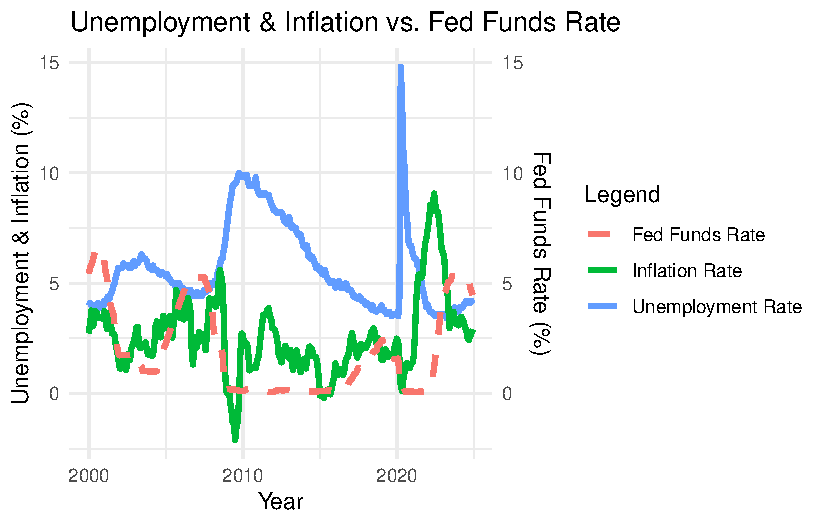
\includegraphics{Week1_Data608_files/figure-latex/unnamed-chunk-25-1.pdf}

Interpretation:

Green bars (``Yes'') → States where funding aligns with population.

Yellow bars (``No'') → States overfunded or underfunded, indicating
inequity.

If many states are yellow, the allocation is not equitable.

\subsubsection{Funding vs.~Population
Percentage}\label{funding-vs.-population-percentage}

If funding is fair, points should align in a linear trend.

\begin{Shaded}
\begin{Highlighting}[]
\FunctionTok{ggplot}\NormalTok{(new\_df, }\FunctionTok{aes}\NormalTok{(}\AttributeTok{x =}\NormalTok{ population\_per\_state\_percentage, }
                   \AttributeTok{y =}\NormalTok{ funding\_per\_state\_percentage, }
                   \AttributeTok{color =}\NormalTok{ Equitable)) }\SpecialCharTok{+}
  \FunctionTok{geom\_point}\NormalTok{(}\AttributeTok{size =} \DecValTok{4}\NormalTok{, }\AttributeTok{alpha =} \FloatTok{0.7}\NormalTok{) }\SpecialCharTok{+}
  \FunctionTok{geom\_smooth}\NormalTok{(}\AttributeTok{method =} \StringTok{"lm"}\NormalTok{, }\AttributeTok{color =} \StringTok{"black"}\NormalTok{, }\AttributeTok{linetype =} \StringTok{"dashed"}\NormalTok{) }\SpecialCharTok{+}
  \FunctionTok{scale\_color\_manual}\NormalTok{(}\AttributeTok{values =} \FunctionTok{c}\NormalTok{(}\StringTok{"Yes"} \OtherTok{=} \StringTok{"green"}\NormalTok{, }\StringTok{"No"} \OtherTok{=} \StringTok{"orange"}\NormalTok{)) }\SpecialCharTok{+}
  \FunctionTok{labs}\NormalTok{(}\AttributeTok{title =} \StringTok{"Funding Allocation vs. Population Percentage"}\NormalTok{,}
       \AttributeTok{x =} \StringTok{"Population Percentage"}\NormalTok{,}
       \AttributeTok{y =} \StringTok{"Funding Percentage"}\NormalTok{,}
       \AttributeTok{color =} \StringTok{"Equitable"}\NormalTok{) }\SpecialCharTok{+}
  \FunctionTok{theme\_minimal}\NormalTok{()}
\end{Highlighting}
\end{Shaded}

\begin{verbatim}
## `geom_smooth()` using formula = 'y ~ x'
\end{verbatim}

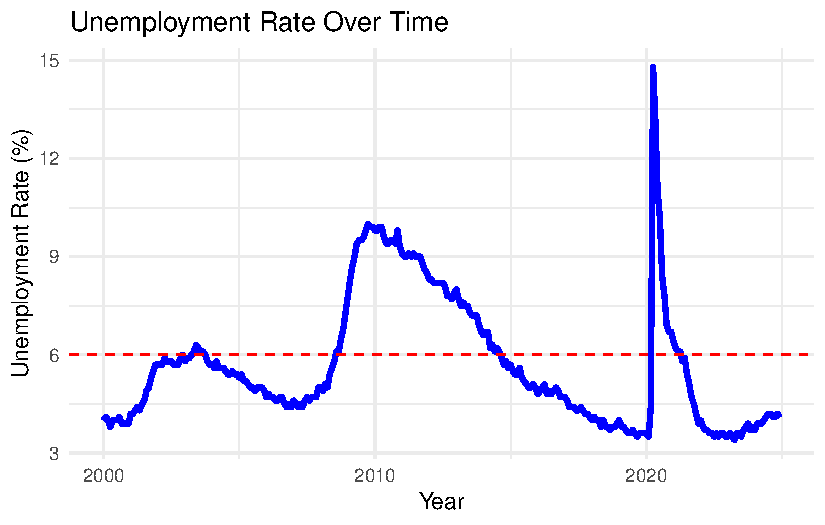
\includegraphics{Week1_Data608_files/figure-latex/unnamed-chunk-26-1.pdf}

Interpretation:

A strong trend line suggests fair allocation.

Scattered points with many ``No'' (yellow) indicate funding was not
proportional.

\subsubsection{Is the allocation equitable based on the population of
each of the States and Territories, or is bias
apparent?}\label{is-the-allocation-equitable-based-on-the-population-of-each-of-the-states-and-territories-or-is-bias-apparent}

According to the chart below, about 80\% of the states have inequitable
allocation.

Does the allocation favor the political interests of the Biden
administration?

No, it doesn't serve the political interests of the Biden administration

\begin{Shaded}
\begin{Highlighting}[]
\FunctionTok{ggplot}\NormalTok{(new\_df, }\FunctionTok{aes}\NormalTok{(}\AttributeTok{x =} \FunctionTok{reorder}\NormalTok{(state\_name, population\_per\_state\_percentage), }
                   \AttributeTok{y =}\NormalTok{ funding\_per\_state\_percentage, }
                   \AttributeTok{fill =}\NormalTok{ bias)) }\SpecialCharTok{+}
  \FunctionTok{geom\_bar}\NormalTok{(}\AttributeTok{stat =} \StringTok{"identity"}\NormalTok{) }\SpecialCharTok{+}
  \FunctionTok{coord\_flip}\NormalTok{() }\SpecialCharTok{+}
  \FunctionTok{scale\_fill\_manual}\NormalTok{(}\AttributeTok{values =} \FunctionTok{c}\NormalTok{(}\StringTok{"Yes"} \OtherTok{=} \StringTok{"orange"}\NormalTok{, }\StringTok{"No"} \OtherTok{=} \StringTok{"green"}\NormalTok{)) }\SpecialCharTok{+}
  \FunctionTok{labs}\NormalTok{(}\AttributeTok{title =} \StringTok{"Funding Allocation vs. Population Percentage"}\NormalTok{,}
       \AttributeTok{x =} \StringTok{"State"}\NormalTok{,}
       \AttributeTok{y =} \StringTok{"Funding Percentage"}\NormalTok{,}
       \AttributeTok{fill =} \StringTok{"bias"}\NormalTok{) }\SpecialCharTok{+}
  \FunctionTok{theme\_minimal}\NormalTok{()}
\end{Highlighting}
\end{Shaded}

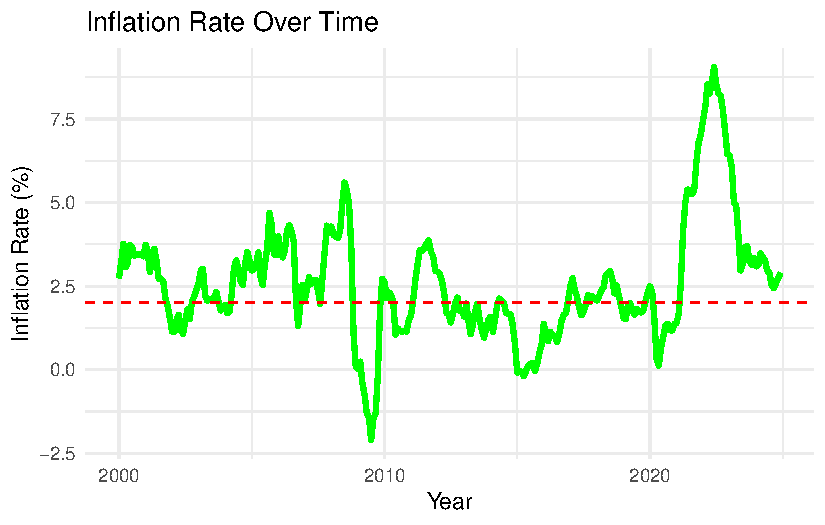
\includegraphics{Week1_Data608_files/figure-latex/unnamed-chunk-27-1.pdf}

\begin{Shaded}
\begin{Highlighting}[]
\CommentTok{\# Define the file path with filename and extension}
\NormalTok{file\_path }\OtherTok{\textless{}{-}} \StringTok{"C:/Users/Uzma/Downloads/new\_df.csv"}

\CommentTok{\# Write dataframe to CSV}
\FunctionTok{write.csv}\NormalTok{(new\_df, }\AttributeTok{file =}\NormalTok{ file\_path, }\AttributeTok{row.names =} \ConstantTok{FALSE}\NormalTok{)}

\CommentTok{\# Confirm that the file was saved}
\FunctionTok{print}\NormalTok{(}\StringTok{"File saved successfully!"}\NormalTok{)}
\end{Highlighting}
\end{Shaded}

\begin{verbatim}
## [1] "File saved successfully!"
\end{verbatim}

\begin{Shaded}
\begin{Highlighting}[]
\CommentTok{\# Select specific columns}
\NormalTok{group\_df }\OtherTok{\textless{}{-}}\NormalTok{ new\_df }\SpecialCharTok{\%\textgreater{}\%} \FunctionTok{select}\NormalTok{(state\_name, funding\_billions, popestimate2020, trump\_win, biden\_win)}

\CommentTok{\# View the new data frame}
\DocumentationTok{\#\#\#print(group\_df)}
\end{Highlighting}
\end{Shaded}

\begin{Shaded}
\begin{Highlighting}[]
\CommentTok{\# Calculate total funding and population}
\NormalTok{total\_funding }\OtherTok{\textless{}{-}} \FunctionTok{sum}\NormalTok{(group\_df}\SpecialCharTok{$}\NormalTok{funding\_billions, }\AttributeTok{na.rm =} \ConstantTok{TRUE}\NormalTok{)}
\NormalTok{total\_population }\OtherTok{\textless{}{-}} \FunctionTok{sum}\NormalTok{(group\_df}\SpecialCharTok{$}\NormalTok{popestimate2020, }\AttributeTok{na.rm =} \ConstantTok{TRUE}\NormalTok{)}

\CommentTok{\# Create a new table with grouped states and percentages}
\NormalTok{grouped\_table }\OtherTok{\textless{}{-}}\NormalTok{ group\_df }\SpecialCharTok{\%\textgreater{}\%}
  \FunctionTok{group\_by}\NormalTok{(trump\_win, biden\_win) }\SpecialCharTok{\%\textgreater{}\%}
  \FunctionTok{summarize}\NormalTok{(}
    \AttributeTok{trump\_funding\_percentage =} \FunctionTok{round}\NormalTok{(}\FunctionTok{sum}\NormalTok{(}\FunctionTok{ifelse}\NormalTok{(trump\_win }\SpecialCharTok{==} \DecValTok{1}\NormalTok{, funding\_billions, }\DecValTok{0}\NormalTok{), }\AttributeTok{na.rm =} \ConstantTok{TRUE}\NormalTok{) }\SpecialCharTok{/}\NormalTok{ total\_funding }\SpecialCharTok{*} \DecValTok{100}\NormalTok{, }\DecValTok{2}\NormalTok{),}
    \AttributeTok{biden\_funding\_percentage =} \FunctionTok{round}\NormalTok{(}\FunctionTok{sum}\NormalTok{(}\FunctionTok{ifelse}\NormalTok{(biden\_win }\SpecialCharTok{==} \DecValTok{1}\NormalTok{, funding\_billions, }\DecValTok{0}\NormalTok{), }\AttributeTok{na.rm =} \ConstantTok{TRUE}\NormalTok{) }\SpecialCharTok{/}\NormalTok{ total\_funding }\SpecialCharTok{*} \DecValTok{100}\NormalTok{, }\DecValTok{2}\NormalTok{),}
    \AttributeTok{trump\_population\_percentage =} \FunctionTok{round}\NormalTok{(}\FunctionTok{sum}\NormalTok{(}\FunctionTok{ifelse}\NormalTok{(trump\_win }\SpecialCharTok{==} \DecValTok{1}\NormalTok{, popestimate2020, }\DecValTok{0}\NormalTok{), }\AttributeTok{na.rm =} \ConstantTok{TRUE}\NormalTok{) }\SpecialCharTok{/}\NormalTok{ total\_population }\SpecialCharTok{*} \DecValTok{100}\NormalTok{, }\DecValTok{2}\NormalTok{),}
    \AttributeTok{biden\_population\_percentage =} \FunctionTok{round}\NormalTok{(}\FunctionTok{sum}\NormalTok{(}\FunctionTok{ifelse}\NormalTok{(biden\_win }\SpecialCharTok{==} \DecValTok{1}\NormalTok{, popestimate2020, }\DecValTok{0}\NormalTok{), }\AttributeTok{na.rm =} \ConstantTok{TRUE}\NormalTok{) }\SpecialCharTok{/}\NormalTok{ total\_population }\SpecialCharTok{*} \DecValTok{100}\NormalTok{, }\DecValTok{2}\NormalTok{)}
\NormalTok{  ) }\SpecialCharTok{\%\textgreater{}\%}
  \FunctionTok{ungroup}\NormalTok{()}
\end{Highlighting}
\end{Shaded}

\begin{verbatim}
## `summarise()` has grouped output by 'trump_win'. You can override using the
## `.groups` argument.
\end{verbatim}

\begin{Shaded}
\begin{Highlighting}[]
\CommentTok{\# Print the new grouped table with rounded percentages}
\FunctionTok{print}\NormalTok{(grouped\_table)}
\end{Highlighting}
\end{Shaded}

\begin{verbatim}
## # A tibble: 2 x 6
##   trump_win biden_win trump_funding_percentage biden_funding_percentage
##       <int>     <int>                    <dbl>                    <dbl>
## 1         0         1                      0                       53.6
## 2         1         0                     46.4                      0  
## # i 2 more variables: trump_population_percentage <dbl>,
## #   biden_population_percentage <dbl>
\end{verbatim}

\begin{Shaded}
\begin{Highlighting}[]
\CommentTok{\# Define the file path with filename and extension}
\NormalTok{file\_path }\OtherTok{\textless{}{-}} \StringTok{"C:/Users/Uzma/Downloads/grouped\_table.csv"}

\CommentTok{\# Write dataframe to CSV}
\FunctionTok{write.csv}\NormalTok{(grouped\_table, }\AttributeTok{file =}\NormalTok{ file\_path, }\AttributeTok{row.names =} \ConstantTok{FALSE}\NormalTok{)}

\CommentTok{\# Confirm that the file was saved}
\FunctionTok{print}\NormalTok{(}\StringTok{"File saved successfully!"}\NormalTok{)}
\end{Highlighting}
\end{Shaded}

\begin{verbatim}
## [1] "File saved successfully!"
\end{verbatim}

\subsubsection{Does the allocation favor the political interests of the
Biden
administration?}\label{does-the-allocation-favor-the-political-interests-of-the-biden-administration}

No, it does not favor the the political interests of the Biden
administration.

\subsubsection{Comparing Funding vs.~Population
Distribution}\label{comparing-funding-vs.-population-distribution}

\subsubsection{Bar Chart}\label{bar-chart}

\begin{Shaded}
\begin{Highlighting}[]
\CommentTok{\# Convert data to long format for easy visualization}
\NormalTok{grouped\_long }\OtherTok{\textless{}{-}}\NormalTok{ grouped\_table }\SpecialCharTok{\%\textgreater{}\%}
  \FunctionTok{pivot\_longer}\NormalTok{(}\AttributeTok{cols =} \FunctionTok{c}\NormalTok{(trump\_funding\_percentage, biden\_funding\_percentage, }
\NormalTok{                        trump\_population\_percentage, biden\_population\_percentage), }
               \AttributeTok{names\_to =} \StringTok{"Category"}\NormalTok{, }
               \AttributeTok{values\_to =} \StringTok{"Percentage"}\NormalTok{)}

\CommentTok{\# Create labels for clarity}
\NormalTok{grouped\_long}\SpecialCharTok{$}\NormalTok{Group }\OtherTok{\textless{}{-}} \FunctionTok{ifelse}\NormalTok{(}\FunctionTok{grepl}\NormalTok{(}\StringTok{"trump"}\NormalTok{, grouped\_long}\SpecialCharTok{$}\NormalTok{Category), }\StringTok{"Trump{-}Won States"}\NormalTok{, }\StringTok{"Biden{-}Won States"}\NormalTok{)}
\NormalTok{grouped\_long}\SpecialCharTok{$}\NormalTok{Metric }\OtherTok{\textless{}{-}} \FunctionTok{ifelse}\NormalTok{(}\FunctionTok{grepl}\NormalTok{(}\StringTok{"funding"}\NormalTok{, grouped\_long}\SpecialCharTok{$}\NormalTok{Category), }\StringTok{"Funding Allocation"}\NormalTok{, }\StringTok{"Population Percentage"}\NormalTok{)}

\CommentTok{\# Create the bar chart}
\FunctionTok{ggplot}\NormalTok{(grouped\_long, }\FunctionTok{aes}\NormalTok{(}\AttributeTok{x =}\NormalTok{ Group, }\AttributeTok{y =}\NormalTok{ Percentage, }\AttributeTok{fill =}\NormalTok{ Metric)) }\SpecialCharTok{+}
  \FunctionTok{geom\_bar}\NormalTok{(}\AttributeTok{stat =} \StringTok{"identity"}\NormalTok{, }\AttributeTok{position =} \StringTok{"dodge"}\NormalTok{) }\SpecialCharTok{+}
  \FunctionTok{scale\_fill\_manual}\NormalTok{(}\AttributeTok{values =} \FunctionTok{c}\NormalTok{(}\StringTok{"Funding Allocation"} \OtherTok{=} \StringTok{"green"}\NormalTok{, }\StringTok{"Population Percentage"} \OtherTok{=} \StringTok{"orange"}\NormalTok{)) }\SpecialCharTok{+}
  \FunctionTok{labs}\NormalTok{(}\AttributeTok{title =} \StringTok{"Funding Allocation vs. Population Share by Political Affiliation"}\NormalTok{,}
       \AttributeTok{x =} \StringTok{"Political Affiliation (2020 Election)"}\NormalTok{,}
       \AttributeTok{y =} \StringTok{"Percentage of Total"}\NormalTok{,}
       \AttributeTok{fill =} \StringTok{"Category"}\NormalTok{) }\SpecialCharTok{+}
  \FunctionTok{theme\_minimal}\NormalTok{()}
\end{Highlighting}
\end{Shaded}

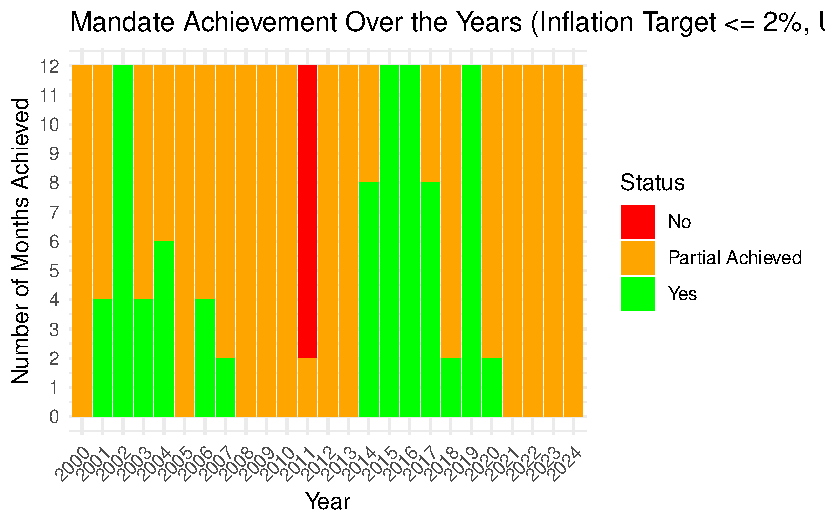
\includegraphics{Week1_Data608_files/figure-latex/unnamed-chunk-32-1.pdf}

Analysis of the Bar Chart

If funding allocation closely matches population share, then the
distribution is likely fair.

If Biden states receive significantly more funding than their population
share, it suggests possible bias in allocation.

If Trump states receive less funding despite a larger population share,
it may indicate under funding relative to need.

\subsubsection{Funding vs.~Population for Biden vs.~Trump
States}\label{funding-vs.-population-for-biden-vs.-trump-states}

This scatter plot shows whether Biden states received disproportionately
more funding.

\subsubsection{Scatter Plot}\label{scatter-plot}

\begin{Shaded}
\begin{Highlighting}[]
\FunctionTok{ggplot}\NormalTok{(grouped\_table, }\FunctionTok{aes}\NormalTok{(}\AttributeTok{x =}\NormalTok{ trump\_population\_percentage, }\AttributeTok{y =}\NormalTok{ trump\_funding\_percentage, }\AttributeTok{color =} \StringTok{"Trump States"}\NormalTok{)) }\SpecialCharTok{+}
  \FunctionTok{geom\_point}\NormalTok{(}\AttributeTok{size =} \DecValTok{4}\NormalTok{) }\SpecialCharTok{+}
  \FunctionTok{geom\_smooth}\NormalTok{(}\AttributeTok{method =} \StringTok{"lm"}\NormalTok{, }\AttributeTok{linetype =} \StringTok{"dashed"}\NormalTok{, }\AttributeTok{color =} \StringTok{"red"}\NormalTok{) }\SpecialCharTok{+}
  \FunctionTok{geom\_point}\NormalTok{(}\FunctionTok{aes}\NormalTok{(}\AttributeTok{x =}\NormalTok{ biden\_population\_percentage, }\AttributeTok{y =}\NormalTok{ biden\_funding\_percentage, }\AttributeTok{color =} \StringTok{"Biden States"}\NormalTok{), }\AttributeTok{size =} \DecValTok{4}\NormalTok{) }\SpecialCharTok{+}
  \FunctionTok{geom\_smooth}\NormalTok{(}\FunctionTok{aes}\NormalTok{(}\AttributeTok{x =}\NormalTok{ biden\_population\_percentage, }\AttributeTok{y =}\NormalTok{ biden\_funding\_percentage), }
              \AttributeTok{method =} \StringTok{"lm"}\NormalTok{, }\AttributeTok{linetype =} \StringTok{"dashed"}\NormalTok{, }\AttributeTok{color =} \StringTok{"blue"}\NormalTok{) }\SpecialCharTok{+}
  \FunctionTok{scale\_color\_manual}\NormalTok{(}\AttributeTok{values =} \FunctionTok{c}\NormalTok{(}\StringTok{"Trump States"} \OtherTok{=} \StringTok{"red"}\NormalTok{, }\StringTok{"Biden States"} \OtherTok{=} \StringTok{"blue"}\NormalTok{)) }\SpecialCharTok{+}
  \FunctionTok{labs}\NormalTok{(}\AttributeTok{title =} \StringTok{"Funding Allocation vs. Population Share for Trump and Biden States"}\NormalTok{,}
       \AttributeTok{x =} \StringTok{"Population Share (\%)"}\NormalTok{,}
       \AttributeTok{y =} \StringTok{"Funding Share (\%)"}\NormalTok{,}
       \AttributeTok{color =} \StringTok{"Political Group"}\NormalTok{) }\SpecialCharTok{+}
  \FunctionTok{theme\_minimal}\NormalTok{()}
\end{Highlighting}
\end{Shaded}

\begin{verbatim}
## `geom_smooth()` using formula = 'y ~ x'
\end{verbatim}

\begin{verbatim}
## Warning in qt((1 - level)/2, df): NaNs produced
\end{verbatim}

\begin{verbatim}
## `geom_smooth()` using formula = 'y ~ x'
\end{verbatim}

\begin{verbatim}
## Warning in qt((1 - level)/2, df): NaNs produced
\end{verbatim}

\begin{verbatim}
## Warning in max(ids, na.rm = TRUE): no non-missing arguments to max; returning
## -Inf

## Warning in max(ids, na.rm = TRUE): no non-missing arguments to max; returning
## -Inf
\end{verbatim}

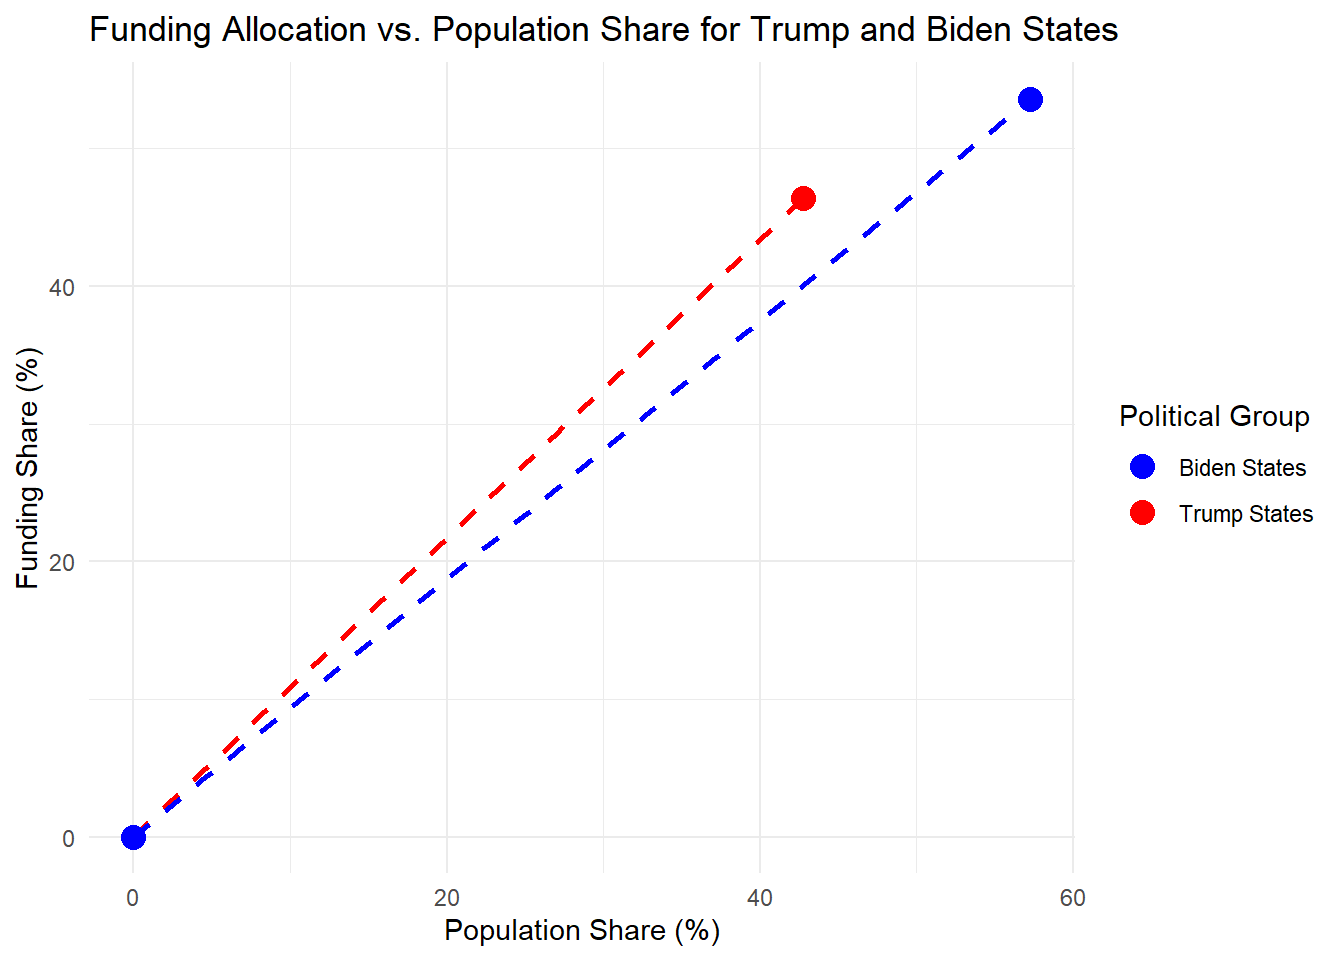
\includegraphics{Week1_Data608_files/figure-latex/unnamed-chunk-33-1.pdf}

\end{document}
